\section{Introduction}

Automatic differentiation has contributed to the rapid pace of innovation in the field of deep learning. Software packages such as PyTorch \citep{pytorch} and Theano \citep{theano} have advanced a programming paradigm where the user (1) defines a neural network architecture by composing differentiable operators and (2) supplies training data. The package then automatically computes the gradient of the error on the training data via recursive application of the chain rule. At this point, the user must become involved again by (3) selecting one of numerous optimisation algorithms and (4) manually tuning its hyperparameters: in particular, the initial learning rate and the learning rate decay schedule \citep{Goodfellow-et-al-2016}.

But manually tuning hyperparameters is irksome. An abundance of hyperparameters makes it difficult to rank the performance of different deep learning algorithms \citep{Lucic2017AreGC,crowded_valley} and difficult to reproduce results in the literature \citep{deeprlmatters}. Hyperparameters confound our efforts to build a scientific understanding of generalisation in deep learning \citep{jiang2019fantastic, my-margin}. And, when training neural networks at the largest scale, in pursuit of stronger forms of artificial intelligence, hyperparameter grid search can rack up millions of dollars in compute costs \citep{Sharir2020TheCO}. 

Are hyperparameters just a fact of life? The thesis of this paper is that \textit{no: they are not}. Deep learning involves fitting a known function to known data via minimising a known objective. If we could characterise these components both individually and in how they interact, then---in principle---there should be no leftover degrees of freedom to be tuned \citep{tutorial}. Taking this idea and running with it leads to \textit{automatic gradient descent} (AGD): a neural network optimiser without any hyperparameters. AGD is complementary to automatic differentiation and could help to automate general machine learning workflows.

Two existing tools are central to our derivation, and it is their novel combination that presents the main theoretical contribution of this paper. First, a classic tool from convex analysis known as the \textit{Bregman divergence} \citep{bregman1967relaxation,bregman} is used to characterise how the neural network interacts with the loss function. And second, a tool called \textit{deep relative trust} \citep{my-fromage} is used to characterise the highly non-linear interaction between the weights and the network output. With these tools in hand, we can apply the \textit{majorise-minimise meta-algorithm} \citep{mm} to derive an optimiser explicitly tailored to deep network objective functions. To summarise, the derivation of AGD follows three main steps:

\begin{enumerate}[label=Step \arabic*:, leftmargin=*, font=\sffamily]
    \item \textsf{Functional expansion}. We use a \textit{Bregman divergence} to express the linearisation error of the objective function $\el(\vw)$ in terms of the functional perturbation $\Delta \vf$ to the network $\vf$.
    \item \textsf{Architectural perturbation bounds.} We use \textit{deep relative trust} to relate the size and structure of the weight perturbation $\Delta \vw$ to the size of the induced functional perturbation $\Delta \vf$.
    \item \textsf{Majorise-minimise.} We substitute deep relative trust into the Bregman divergence to obtain an explicitly architecture-dependent majorisation. Minimising with respect to $\Delta \vw$ yields an optimiser.
\end{enumerate}

\paragraph{Summary of contributions} This paper derives automatic gradient descent (AGD) by applying the majorise-minimise meta-algorithm to deep network objective functions. AGD trains all tested network architectures without hyperparameters, and scales to deep networks such as ResNet-50 and large datasets such as ImageNet. AGD trains out-of-the-box even when Adam and SGD fail to train with their default hyperparameters.

\begin{table}
    \centering
    \begin{tabularx}{\textwidth}{lXccccc}
        \toprule
        \textbf{Optimiser} &
        \textbf{Reference} & 
        \makecell{\textbf{Hyperparameter}\\\textbf{Free}} &
        \makecell{\textbf{Width}\\\textbf{Scaling}} & \makecell{\textbf{Depth}\\\textbf{Scaling}} &  
        \makecell{\textbf{Automatic}\\\textbf{Schedule}} & 
        \makecell{\textbf{Memory}\\\textbf{Cost}} \\ 
        \midrule
        Adam    & $\mathrlap{\text{\citet{kingma_adam:_2015}}}$ & \xmark & \xmark & \xmark & \xmark & $3 \times \#$weights\\
        SGD + mom.     & $\mathrlap{\text{\citet{bottou}}}$ & \xmark & \xmark & \xmark & \xmark & $2\times\#$weights\\
        SGD + muP     & $\mathrlap{\text{\citet{Yang2021TensorPI}}}$ & \xmark & \cmark & \xmark & \xmark & $1\times\#$weights\\
        AGD     & this paper                & \cmark & \cmark & \cmark & \cmark & $1\times\#$weights\\ 
        \bottomrule
    \end{tabularx}
    \caption{\captiontitle{Comparing practical optimisers.} Adam and momentum-SGD employ running estimates of gradient statistics and thereby use more memory than AGD. In addition, Adam and SGD do not provide guidance on scaling hyperparameters with network architecture, although muP fixes this for the case of width scaling.}
    \label{tab:practice}
\end{table}

\subsection{Related work}

\paragraph{Optimisation theory} First-order optimisers leverage the first-order Taylor expansion of the objective function $\el(\vw)$---in particular, the gradient $\nabla_\vw\el(\vw)$. Theoretical treatments include mirror descent \citep{nemirovsky_yudin_1983}, 
natural gradient descent \citep{amari} and the Gauss-Newton method \citep{gauss-newton}. These methods have been explored in the context of deep learning \citep{revisiting-ngd,azizan2018stochastic,sun2022mirror}. First-order methods are amenable to deep learning since the gradient of the objective is available via recursive application of the chain rule---a.k.a.\ error back-propagation \citep{Rumelhart1986LearningRB}.

Second-order optimisers leverage the second-order Taylor expansion of the objective function $\el(\vw)$---in particular, the gradient $\nabla_\vw\el(\vw)$ and Hessian $\nabla^2_\vw\el(\vw)$. Examples include Newton's method \citep{Nocedal1999NumericalO} and cubic-regularised Newton's method \citep{Nesterov2006CubicRO}. Naïvely, second-order methods are less amenable to deep learning since the cost of the relevant Hessian computations is prohibitive at high dimension. That being said, efforts have been made to circumvent this issue \citep{hessian-linear}.

The majorise-minimise meta-algorithm \citep{mm} is an algorithmic pattern that can be used to derive optimisers. To apply the meta-algorithm, one must first derive an upper bound on the objective which matches the objective up to $k$th-order in its Taylor series for some integer $k$. This \textit{majorisation} can then be minimised as a proxy for reducing the original objective. \cref{fig:maj-min} illustrates the meta-algorithm for $k=1$.

\paragraph{Deep learning theory} The \textit{Lipschitz smoothness assumption}---a global constraint on the eigenvalues of the Hessian---is often used to derive and analyse neural network optimisers \citep{Agarwal2016FindingAL}. But this assumption has been questioned \citep{Zhang2020Why} and evidence has even been found for the reverse relationship, where the Hessian spectrum is highly sensitive to the choice of optimiser \citep{cohen2021gradient}.

These considerations motivate the development of theory that is more explicitly tailored to neural architecture. For instance, \citet{my-fromage} used an architectural perturbation bound termed \textit{deep relative trust} to characterise the neural network optimisation landscape as a function of network depth. Similarly, \citet{Yang2021TensorPI} sought to understand the role of width, leading to their \textit{maximal update parameterisation}. \cref{tab:practice,tab:theory} provide some points of comparison between automatic gradient descent and these and other frameworks.

\begin{figure}
\begin{minipage}{\textwidth}
\centering
\raisebox{-0.5\height}{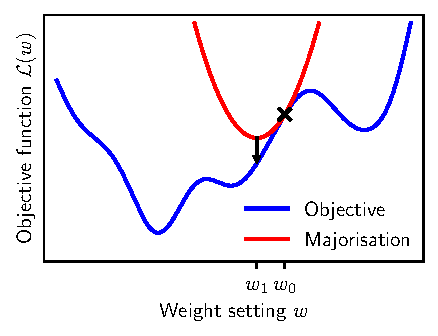
\includegraphics{figures/pdf/maj-min}} \hfill     \raisebox{-0.5\height}{
        \begin{tikzpicture}
        [thick, block/.style={draw, minimum size=1.1cm}]
        
        \node [block,fill=red!30]    (a)               {$\el$};
        \node [block,fill=green!30]  (b) [right =of a] {$\ell$};
        \node [block,fill=orange!30] (c) [right =of b] {$\vf$};
        \node [block,fill=blue!30]   (d) [right =of c] {$\vw$};
        
        \node [block,fill=red!10]    (u) [below =of a] {$\Delta \el$};
        \node [block,fill=green!10]  (v) [below =of b] {$\Delta \ell$};
        \node [block,fill=orange!10] (w) [below =of c] {$\Delta \vf$};
        \node [block,fill=blue!10]   (x) [above =of d] {$\Delta \vw$};
        
        \node (p) [left  =of x, align=right, xshift=0.8cm, yshift=-0.04cm] {perturbation applied\\by optimiser};
        \node (q) [below =of v, yshift=0.9cm, align=center] {$\underbrace{\hspace{14.5em}}$\\[0.5ex]perturbations induced by optimiser};
        \node [below =of d, yshift=0.9cm, align=center] {weights};
        \node [above =of c, yshift=-0.825cm, align=center] {model};
        \node [above =of b, yshift=-0.825cm, align=center] {loss};
        \node [above =of a, yshift=-0.89cm, align=center] {objective};
        
        \draw[-latex] (b) edge (a);
        \draw[-latex] (c) edge (b);
        \draw[-latex] (d) edge (c);
        
        \draw[-latex] (a) edge (u);
        \draw[-latex] (b) edge (v);
        \draw[-latex] (c) edge (w);
        \draw[-latex] (x) edge (d);
        \end{tikzpicture}}
\end{minipage}
\caption{\captiontitle{Majorise-minimise and the perturbation hierarchy.} The \captiontitle{left panel} depicts the majorise-minimise meta-algorithm \citep{mm}, which is an algorithmic pattern for reducing an objective (blue) by minimising a sequence of upper bounds (one shown in red). The upper bounds, known as a \textit{majorisation}, must lie tangent to the objective to guarantee an improvement in one step of the meta-algorithm. The \captiontitle{right panel} depicts the perturbation hierarchy of a generic machine learning model: the optimiser perturbs the weights and this induces perturbations to the model output, the loss on individual training examples and ultimately the overall objective. Majorising machine learning objective functions requires addressing the full perturbation hierarchy.}
\label{fig:maj-min}
\end{figure}

\subsection{Preliminaries}

Given a vector $\vv$ in $\R^n$, we will need to measure its size in three different ways:

\begin{definition}[Manhattan norm] The \textit{Manhattan norm} $\norm{\,\cdot\,}_1$ of a vector $\vv$ is defined by $\norm{\vv}_1 \defeq \sum_{i} \abs{\vv_i}$.
\end{definition}

\begin{definition}[Euclidean norm] The \textit{Euclidean norm} $\norm{\,\cdot\,}_2$ of a vector $\vv$ is defined by $\smash{\norm{\vv}_2 \defeq \sqrt{\sum_{i} \vv_i^2}}$.
\end{definition}

\begin{definition}[Infinity norm] The \textit{infinity norm} $\norm{\,\cdot\,}_\infty$ of a vector $\vv$ is defined by $\norm{\vv}_\infty \defeq \max_{i} \abs{\vv_i}$.
\end{definition}

For a matrix $\mM$ in $\R^{m \times n}$, the reader should be aware that it has a singular value decomposition:
\begin{fact}[SVD] Every matrix $\mM$ in $\R^{m\times n}$ admits a \textit{singular value decomposition} (SVD) of the form $\mM = \sum_{i=1}^{\min(m,n)} \sigma_i(\mM) \cdot \vu_i \vv_i^\top$ where the \textit{left singular vectors} $\{\vu_i\}$ are orthonormal vectors in $\R^{m}$, the \textit{right singular vectors} $\{\vv_i\}$ are orthonormal vectors in $\R^{m}$ and the \textit{singular values} $\{\sigma_i(\mM)\}$ are non-negative scalars.
\end{fact}

The singular value decomposition allows us to measure the size of a matrix in two different ways:

\begin{definition}[Frobenius norm] The \textit{Frobenius norm} $\norm{\,\cdot\,}_F$ of a matrix $\mM$ is given by $\norm{\mM}_F \defeq \sqrt{\sum_{i} \sigma_i(\mM)^2}$.
\end{definition}
\begin{definition}[Operator norm] The \textit{operator norm} $\norm{\,\cdot\,}_*$ of a matrix $\mM$ is given by $\norm{\mM}_* \defeq \max_i \sigma_i(\mM)$.
\end{definition}
While the operator norm $\norm{\mM}_*$ reports the largest singular value, the quantity $\norm{\mM}_F / \sqrt{\min(m,n)}$ reports the root mean square singular value. Finally, we will need to understand two aspects of matrix conditioning:
\begin{definition}[Rank] The \textit{rank} of a matrix counts the number of non-zero singular values.
\end{definition}
\begin{definition}[Stable rank]
The \textit{stable rank} of a matrix $\mM$ is defined by $\srank \mM \defeq \norm{\mM}_F^2 / \norm{\mM}_*^2$.
\end{definition}
The stable rank provides an approximation to the rank that ignores the presence of very small singular values. Let us consider the extremes. An orthogonal matrix $\mO\in\R^{m\times n}$ has both full rank and full stable rank: $\rank \mO = \srank \mO = \min(m,n)$. A rank-one matrix $\mP$ has unit stable rank and satisfies $\norm{\mP}_* = \norm{\mP}_F$.